\documentclass{beamer}
\usetheme{Boadilla}
\usecolortheme{beaver}
%\usepackage{graphicx}
%\usepackage{minted}
%\usepackage[numbers]{natbib}
%\usepackage{float}
%\usepackage{multicol}
%\usepackage[magyar]{babel}
\usepackage{hyperref}
\usepackage{multimedia}
%\usepackage{comment}
%\usepackage{ragged2e}

\hypersetup{colorlinks=true, linkcolor=blue, filecolor=magenta, urlcolor=cyan}
\urlstyle{same}

\title{Járművek trajektóriáinak előrejelzése machine learning modellekkel}
\author{Péter Bence Mérnökinformatika BSc 6. félév}%\\Mérnökinformatika BSc 6. félév\\Konzulensek:\\Dr. Horváth András egyetemi docens\\Agg Áron PhD hallgató}
\institute{Széchenyi István University}

\begin{document}

\begin{frame}
\titlepage
\end{frame}

\begin{frame}
\frametitle{Tartalom}
\tableofcontents
\end{frame}

\section{Bevezetés}
\begin{frame}{Bevezetés}
\centering
%\includegraphics[scale=0.3]{deepsort_yolo_figs/gépilátás_modified.jpg}
\movie[showcontrols=true]{\includegraphics[scale=0.3]{../deepsort_yolo_figs/gépilátás_modified.jpg}}{./demo_bevezetes.mp4}
\end{frame}


\section{Objektumdetektálás}
\begin{frame}{Objektumdetektálás}
    \centering
    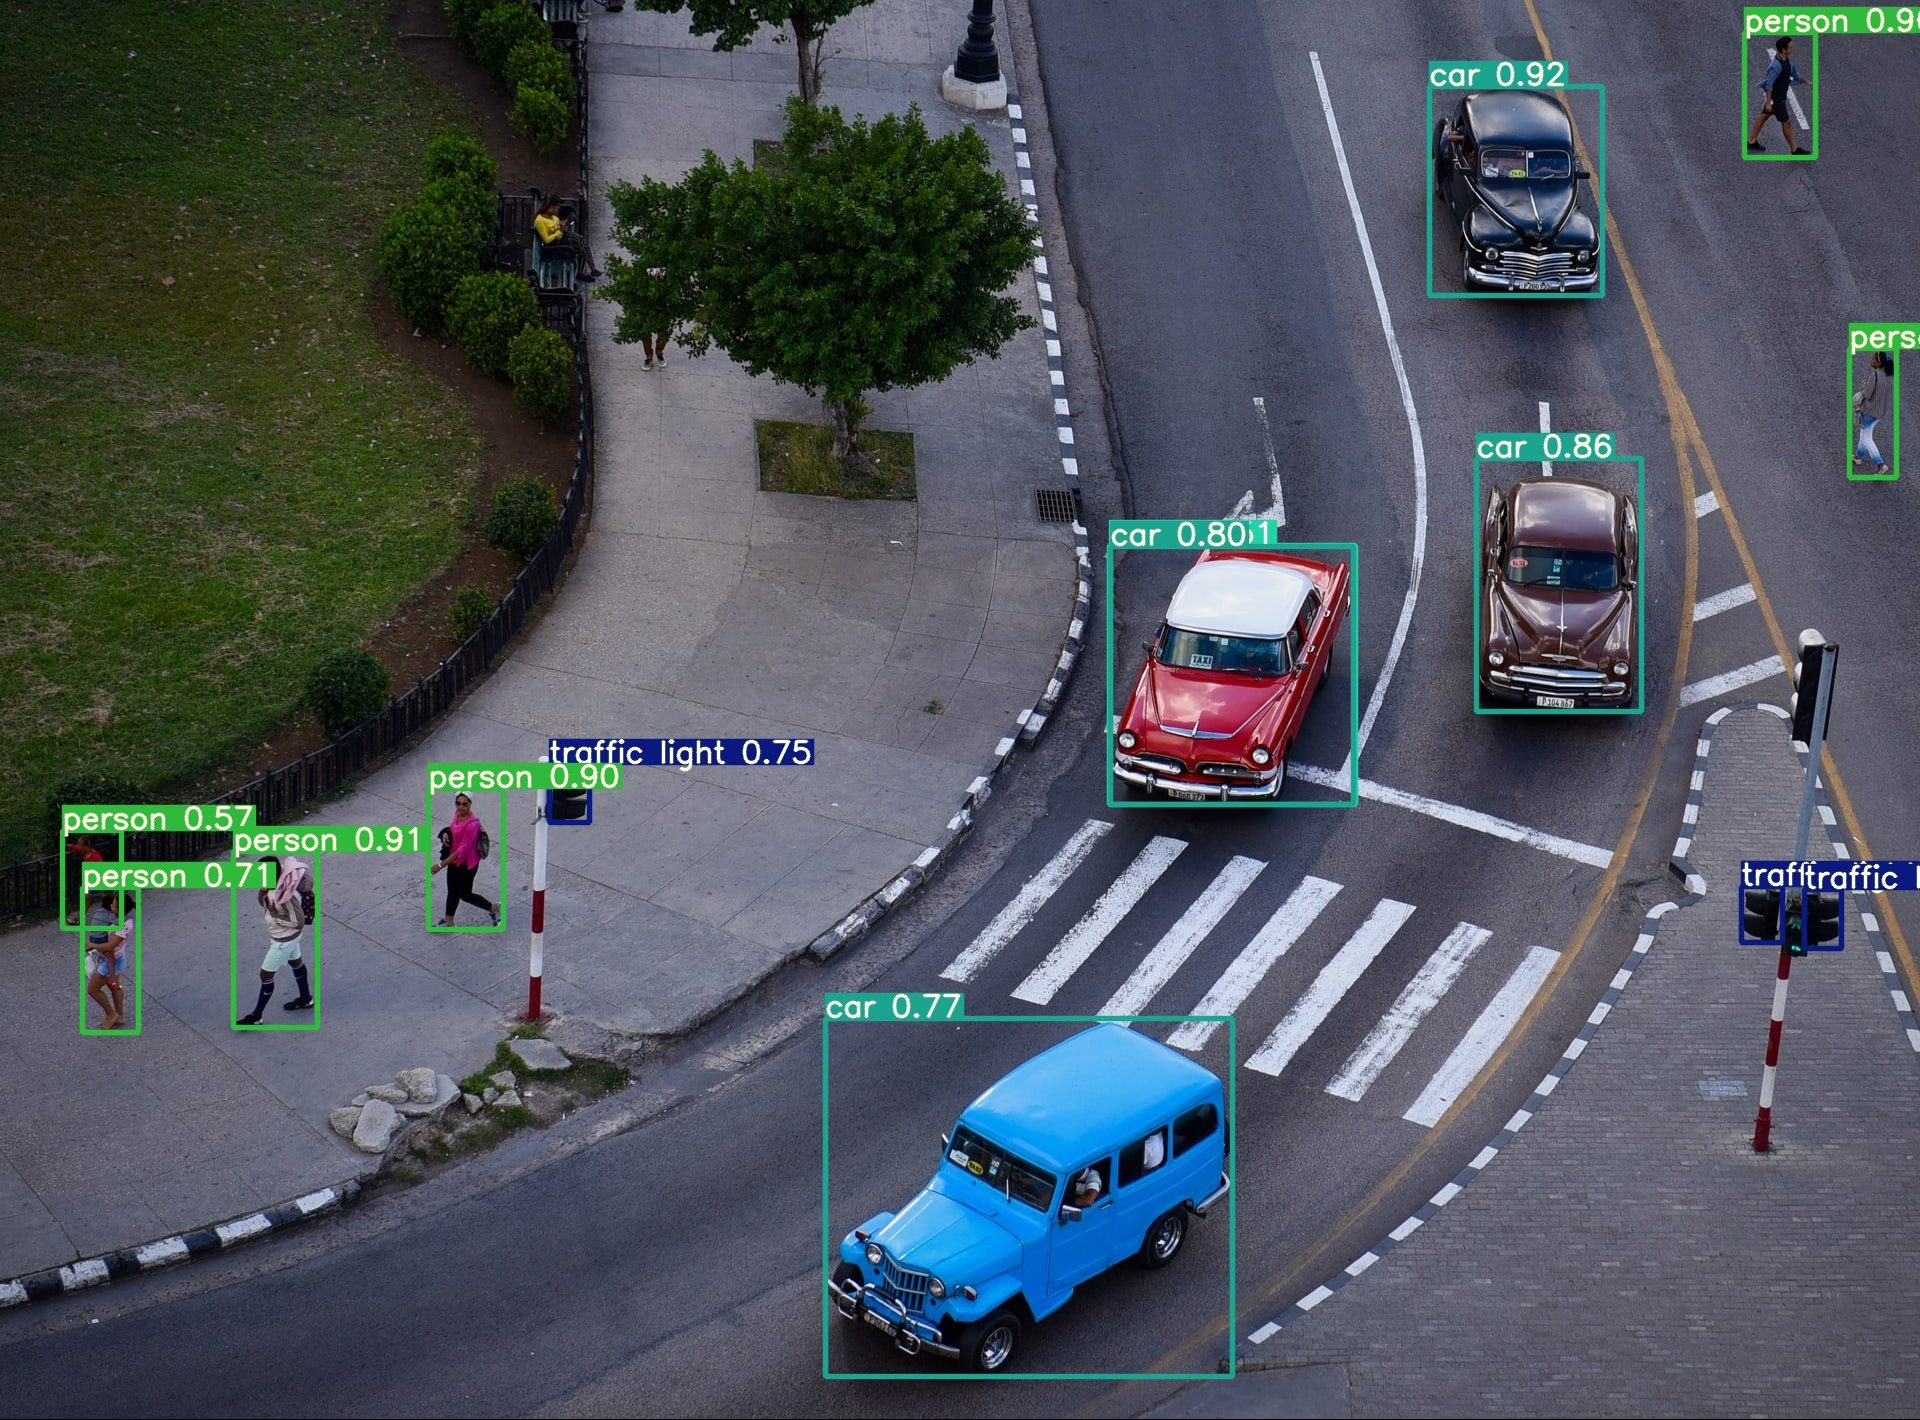
\includegraphics[scale=0.1]{yolo_img.jpg} 
    
\includegraphics[scale=0.1]{yolo_logo.png}
\end{frame}

\section{Objektumkövetés}
\begin{frame}{Objektumkövetés}
    \centering
    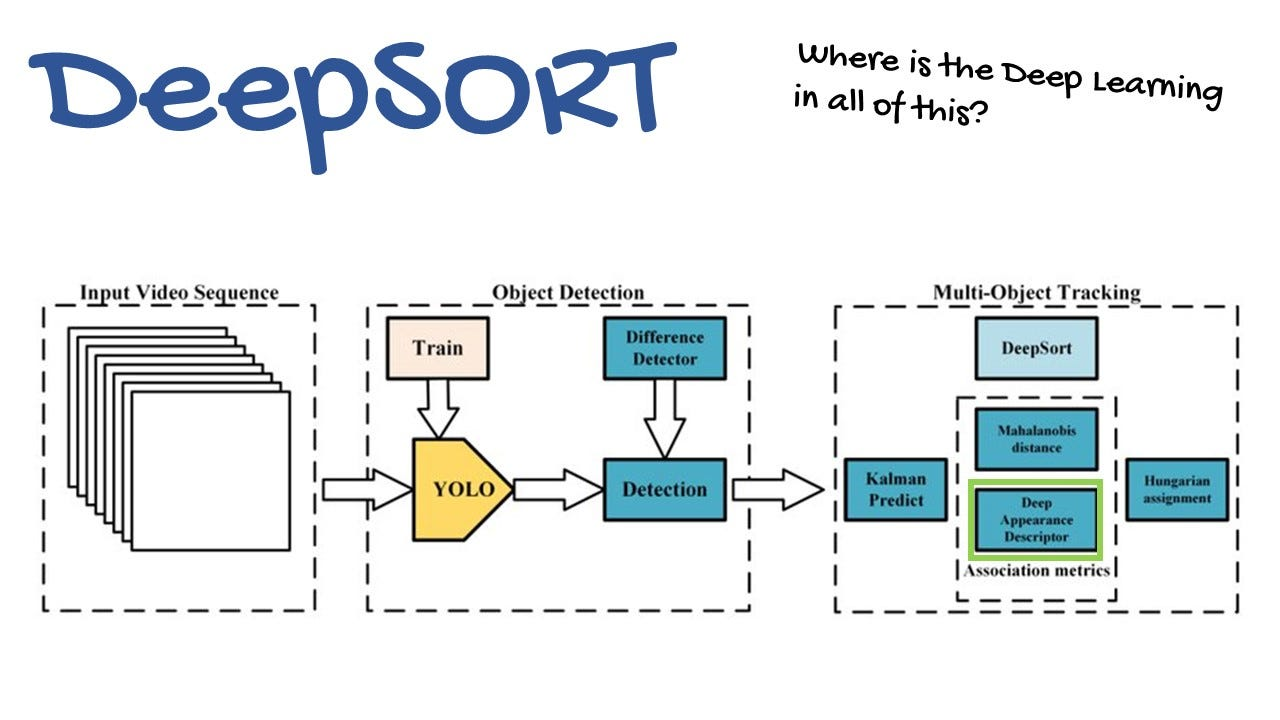
\includegraphics[scale=0.25]{deepsort_flowchart.jpg} 
\end{frame}

\section{Machine Learning}
\begin{frame}{Machine Learning}
    \centering
    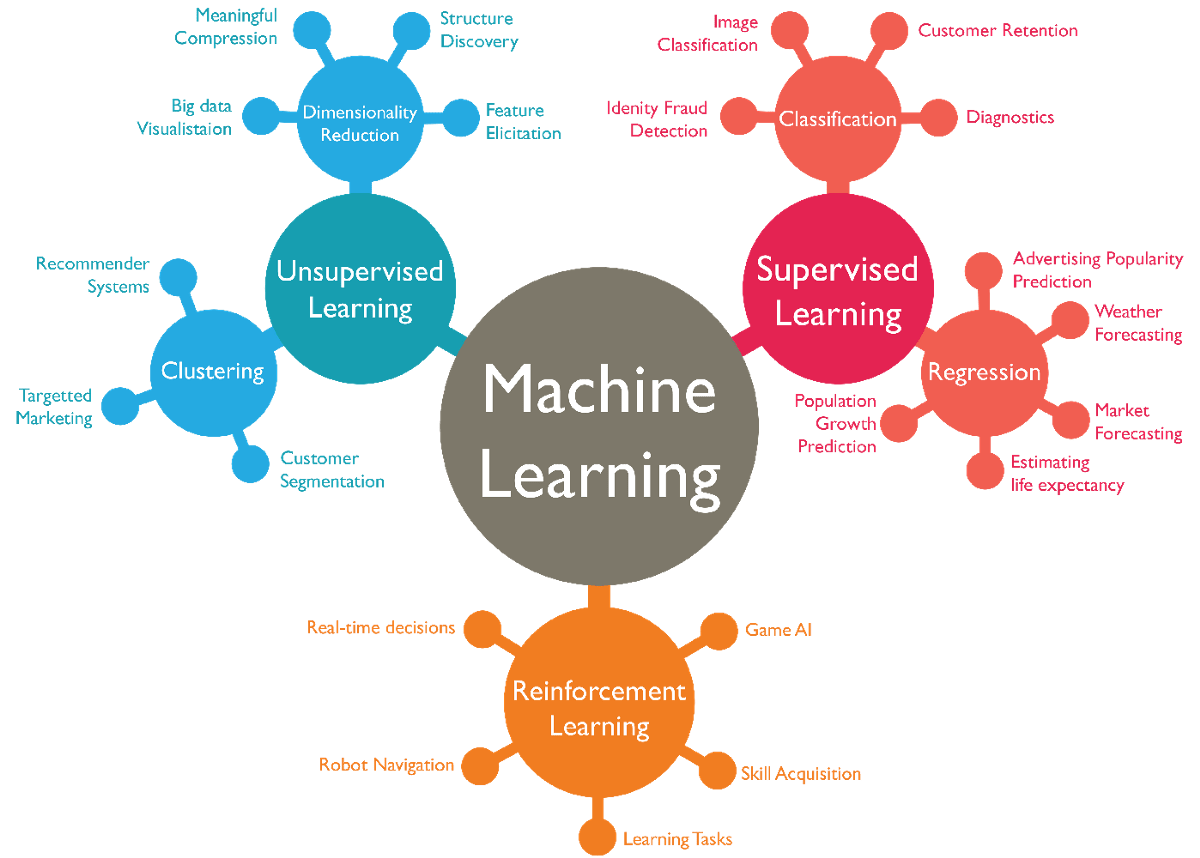
\includegraphics[scale=0.17]{machine_learning.png}    
\end{frame}
\subsection{Unsupervised learning}
\subsection{Supervised Learning}

\section{Klaszterezés}
\begin{frame}{Klaszterezés}

\end{frame}

\section{Klasszifikáció}
\begin{frame}{Klasszifikáció}

\end{frame}



\end{document}